\section{Game Mechanics}
\label{03}

The game we use is called "Robocode"\cite{robocode}. It is a programing game where the players program robots to battle other players' robots. 

Fights between robots take place on a battlefield (see figure \ref{figure-RobocodeBattle01}), which is represented as a Cartesian coordinate system, with (0, 0) being in the lower left corner. Distances are measured in pixels and directions are measured in degrees, where north is 0 degrees, east is 90 degrees, south is 180 degrees and west is 270 degrees. Robots decide on what action they want to take and all robots' actions are then carried out simultaneously.

\begin{figure}[htp]
\centerline{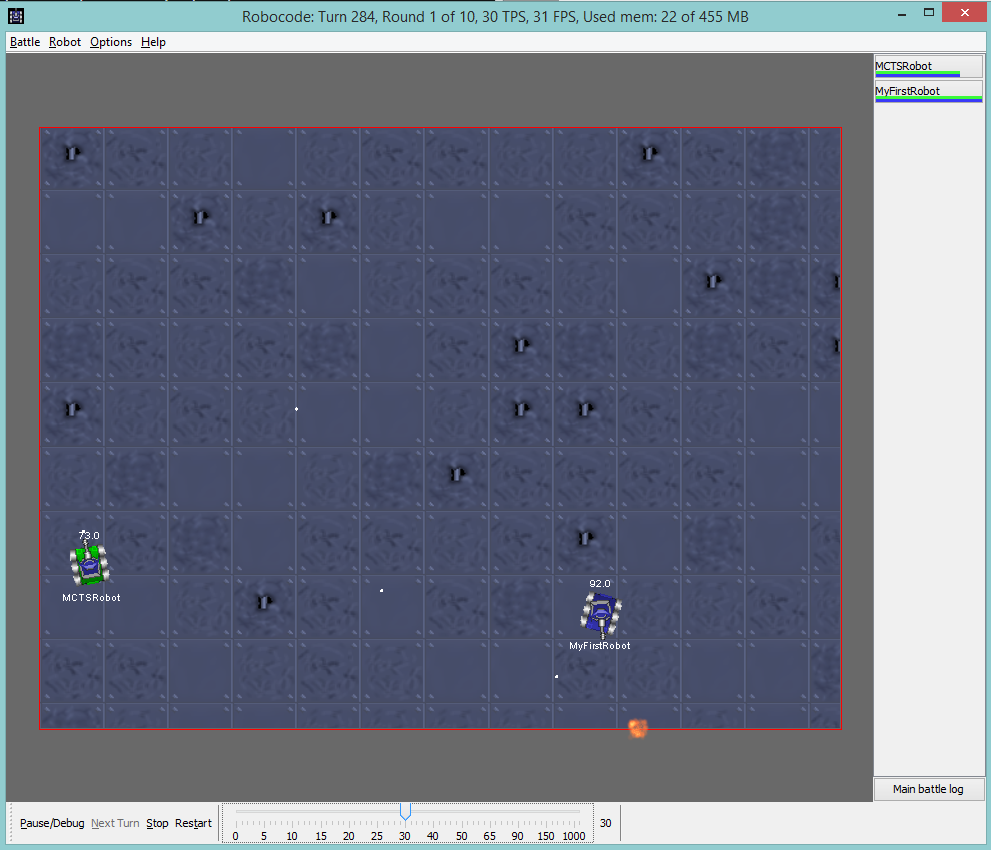
\includegraphics[width=\columnwidth]{Images/RobocodeBattle01}}
\caption{A battle between two robots..}
\label{figure-RobocodeBattle01}
\end{figure}

A robot starts with 100 energy, no idea of where the enemies are and can either move (ahead or back), turn its base, gun or radar or fire its gun during a turn. Moving and turning has no influence on the energy of the robot, but firing the gun and getting hit by bullets decreases its energy. When a robot is out of energy and it is hit by a bullet, it dies. There are limits to how much a robot can move or turn during a single turn\cite{wiki:robocodeGamePhysics} in order to mirror real-life tanks properly.

While a robot is limited to how much it can move or turn during a single turn, its API\cite{robocodeAPI} makes the process easier. For example, if a robot wants to move 100 pixels, it calls the method Ahead(100)\footnote{The Ahead() method takes a double value as parameter, in this case 100.}. This method does not return until the robot has moved the chosen distance, and will thereby prevent other methods from being called meanwhile. As a robot can move no more than 8 pixels per turn, that is, best-case, $\frac{100}{8} = 12.5$ turns in which it only moves, something that is important to keep in mind when designing a robot.

In order to figure out where the enemy is, the robot needs to use its radar. The robot's radar is constantly active and scanning in in a straight line. If an enemy is detected by the radar, which can happen when the radar turns\footnote{The radar is connected to the gun, which is connected to the base of the robot. If one of those turn, the radar turns with them.}, the robot's OnScannedRobot() method is called, even if the robot is moving or turning already. When the OnScannedRobot() method returns, the robot continues doing what it was doing prior to scanning an enemy.

In the OnScannedRobot() method, a robot can take actions as normal. A robot can for example decide to shoot and then move a bit before continuing doing what it was doing before. During this method, a robot has access to some information about the scanned robot, but the information is limited to the following: The enemy robot's heading, velocity and energy, the bearing our gun has and the distance to the enemy. This means that a robot will have to calculate the other robot's position in order to get that information, and that it is impossible to know where another robot's gun is pointing. Considering this, a robot will find it difficult to keep track of what exactly an enemy robot is doing.

Firing the gun is different from moving and turning. Firing the gun can be done with a power level between 1.0 and 3.0. The power level determines how much energy the robot loses (at a 1:1 ratio), and also determines the damage and velocity of the bullet. The more power, the more damage it deals if it hits and the slower the bullet moves. Firing the gun also produces gun heat, and a robot is unable to fire as long as its gun is hot. Gun heat is lowered every turn.

As the gameplay of Robocode consists of developing an AI controller for a robot that does battle with other AI controlled robots, AI is an instrumental tool in making Robocode into what it is.


\subsection{Influence of Robocode mechanics on MCTS}
\label{03_01}

Robocode is, without a doubt, a partially observable game. A robot only knows its own information and occasionally knows where an enemy robot is and where it is heading. There is no way to get any information about the general game state either, so information about where bullets are and where they are heading is completely unavailable.

These factors mean that MCTS has very little information to work with, both during its simulation and its evaluation steps. This will be a challenge, as MCTS will have to make assumptions about where the enemy robot is (even after scanning it, it will quickly move to a new position) and how the enemy behaves in order to be able to simulate a playout and evaluate the results of a playout. If the assumptions are off by just a little, it will have a major impact on how well MCTS performs.